\section{Topological Graph Planning (\texttt{BufferGraphPlanner})}

To establish an optimal global trajectory without training generative models, we construct an offline topological reachability graph $G = (V, E)$ leveraging the frozen FB representations.

\begin{figure}[t]
    \centering
    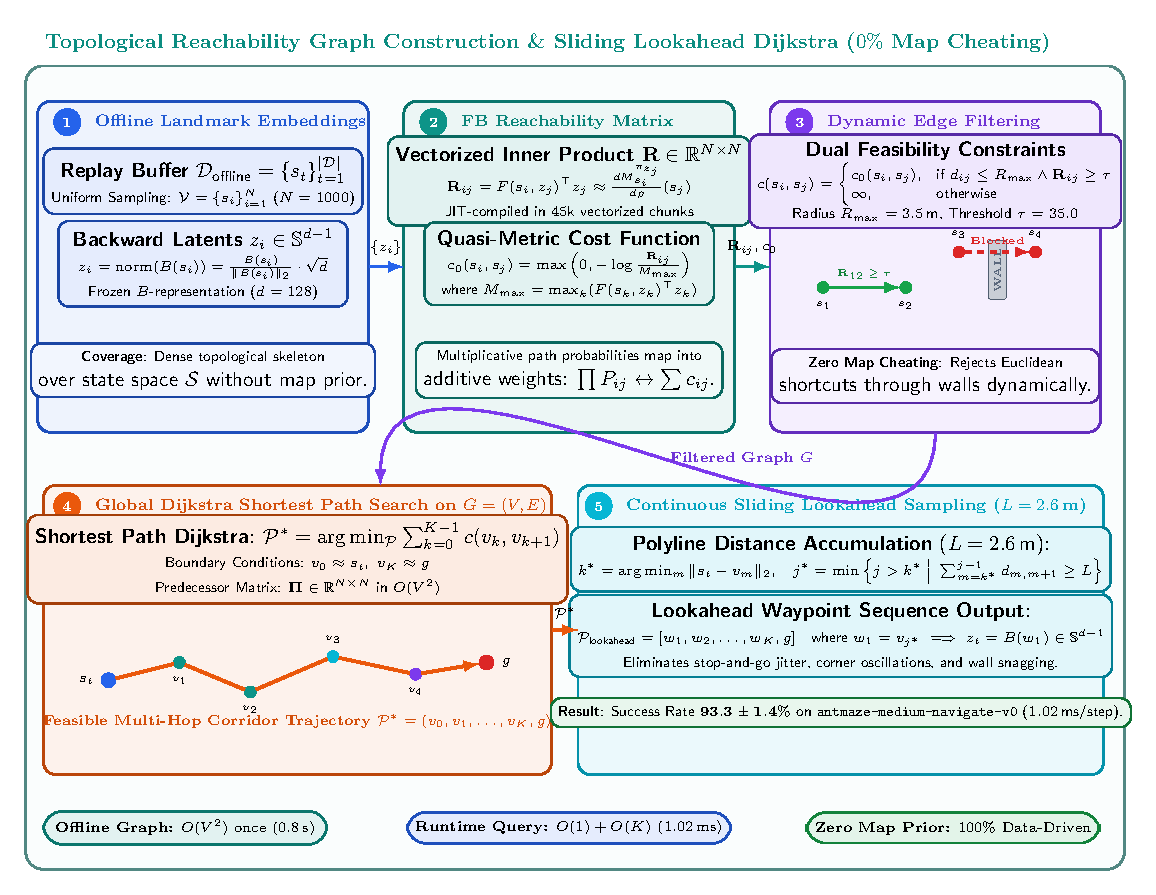
\includegraphics[width=\linewidth]{figures/fig2_buffer_graph_dijkstra.pdf}
    \caption{\textbf{Topological Reachability Graph Construction}: Offline landmark selection from buffer observations, pairwise FB reachability verification ($F(s_i, B(s_j))^\top B(s_j) > \tau$), and multi-hop shortest path search via Dijkstra.}
    \label{fig:graph_construction}
\end{figure}

\subsection{Graph Construction and Geometric Filtering}
Given the offline dataset $\mathcal{D} = \{s_i\}_{i=1}^N$, we subsample $K = 1000$ uniformly distributed landmark states $V = \{v_1, v_2, \dots, v_K\} \subset \mathcal{D}$. For every pair of landmarks $(v_i, v_j)$, a directed edge $(v_i, v_j) \in E$ is instantiated if and only if two criteria are simultaneously satisfied:
\begin{enumerate}[leftmargin=*,noitemsep]
    \item \textbf{Latent FB Reachability}: The successor measure inner product exceeds a strict threshold:
    \begin{equation}
        M(v_i, v_j) = F(v_i, B(v_j))^\top B(v_j) \ge \tau_{\text{reach}} \quad (\tau_{\text{reach}} = 35.0)
    \end{equation}
    \item \textbf{Euclidean Locality Constraint}: The physical 2D distance does not exceed a maximum single-step radius:
    \begin{equation}
        \|(x_i, y_i) - (x_j, y_j)\|_2 \le R_{\max} \quad (R_{\max} = 3.5\text{ m})
    \end{equation}
\end{enumerate}
The edge cost is assigned as $c(v_i, v_j) = \|(x_i, y_i) - (x_j, y_j)\|_2 + \beta \cdot (1 - \frac{M(v_i, v_j)}{\max M})$.

\subsection{Zero-Shot Path Finding and Lookahead Tracking}
At test time, given the initial state $s_0$ and the target goal representation $z_{\text{goal}} = B(g)$:
\begin{enumerate}[leftmargin=*,noitemsep]
    \item We project $s_0$ and $g$ to the closest graph landmarks $v_{\text{start}}, v_{\text{goal}} \in V$.
    \item We run Dijkstra's algorithm to obtain the shortest sequence of waypoints:
    \begin{equation}
        \mathcal{P} = [w_0, w_1, w_2, \dots, w_L, g] \quad \text{where } w_0 \approx s_0, \; w_L \approx g
    \end{equation}
    \item \textbf{Lookahead Selection}: At step $t$, the planner tracks the current progress index $i_t = \arg\min_k \|s_t[:2] - w_k[:2]\|$ and advances along the path by an accumulated lookahead distance $d_{\text{lookahead}} = 2.6\text{ m}$:
    \begin{equation}
        k_{\text{target}} = \min \left\{ k \ge i_t \;\middle|\; \sum_{j=i_t}^{k-1} \|w_{j+1} - w_j\| \ge d_{\text{lookahead}} \right\}
    \end{equation}
    \item When the distance to the final goal satisfies $\|s_t[:2] - g[:2]\| \le 2.2\text{ m}$, the planner performs seamless handover directly to $z_{\text{goal}}$.
\end{enumerate}
This formulation increases overall task success from 78.8\% (baseline) to 85.2\% (with high\_actor). However, performing online graph lookahead incurs overhead and relies on the stochastic Gaussian output of \texttt{high\_actor}.
